\documentclass[11pt]{article}
\usepackage{times}
\usepackage{hyperref}
\usepackage{graphicx}
\usepackage{amsmath}
\usepackage{enumitem}
\usepackage{tikz}
\usetikzlibrary{positioning,fit}

\begin{document}

\title{LLMOps + Enterprise MLOps Modernization}
\author{
  Rohin Solan\thanks{LinkedIn: \href{https://www.linkedin.com/in/rohink}{https://www.linkedin.com/in/rohink}}
}

\date{Sep 2026}
\maketitle


\begin{abstract}
Large Language Models (LLMs) have accelerated enterprise adoption of AI-driven automation, decision intelligence, and knowledge retrieval. However, deploying LLMs reliably, securely, and cost-effectively remains a significant challenge for organizations. This white paper proposes a unified MLOps + LLMOps modernization framework that integrates traditional machine learning lifecycle management with emerging generative AI workflows. Building on prior work such as \textit{EfficientML-Cloud: Hybrid Cost-Aware Inference for Enterprise ML Systems}, this paper extends cost-aware inference, governance, and monitoring principles to LLMs, enabling enterprises to scale AI with confidence.
\end{abstract}

\section{Executive Summary}
Enterprises are rapidly adopting Large Language Models (LLMs) for tasks such as document summarization, customer support automation, code generation, and knowledge retrieval. While LLMs unlock unprecedented capabilities, they also introduce new operational challenges: unpredictable inference costs, hallucination risks, governance gaps, and complex deployment pipelines.

Traditional MLOps frameworks—designed for structured data and supervised learning—are insufficient for managing the lifecycle of LLMs. Enterprises now require a unified operational model that integrates MLOps foundations with LLM-specific workflows such as prompt management, retrieval augmentation, fine-tuning, and hallucination monitoring.

This paper introduces a five-layer modernization framework that unifies MLOps and LLMOps. It extends concepts from the author's prior work, \textit{EfficientML-Cloud}, demonstrating how hybrid cloud/on-prem inference, cost-aware routing, and governance layers can be applied to both ML and LLM systems.

\section{Introduction: The Rise of LLMs in the Enterprise}
The emergence of generative AI has transformed enterprise AI strategies. Unlike traditional ML models, LLMs require:

\begin{itemize}[leftmargin=1.2cm]
    \item Massive compute resources for inference
    \item Complex retrieval pipelines for grounding
    \item Continuous monitoring for hallucinations and toxicity
    \item Governance mechanisms for prompt and output auditing
    \item Specialized deployment strategies across cloud, on-prem, and edge
\end{itemize}

Enterprises face a widening gap between prototype and production. Many organizations successfully build proof-of-concept LLM applications but struggle to operationalize them at scale. Key challenges include:

\begin{itemize}[leftmargin=1.2cm]
    \item High and unpredictable inference costs
    \item Latency variability across cloud providers
    \item Data privacy and regulatory constraints
    \item Lack of reproducibility in prompt-based systems
    \item Difficulty integrating LLMs into existing MLOps pipelines
\end{itemize}

These challenges highlight the need for a unified operational framework that treats LLMs as first-class citizens within enterprise MLOps ecosystems.

\section{Problem Definition: Enterprise Challenges in LLM + ML Lifecycle}
Enterprises must manage both traditional ML models and LLMs simultaneously. This dual landscape introduces challenges across the entire lifecycle.

\subsection{Data and Feature Challenges}
LLMs rely heavily on unstructured data, embeddings, and retrieval pipelines. Enterprises struggle with:

\begin{itemize}[leftmargin=1.2cm]
    \item Inconsistent data ingestion pipelines
    \item Embedding drift over time
    \item Retrieval quality degradation in RAG systems
    \item Lack of versioning for embeddings and vector stores
\end{itemize}

\subsection{Model Management Challenges}
Managing LLMs requires new artifacts beyond traditional ML models:

\begin{itemize}[leftmargin=1.2cm]
    \item Versioning of base models, fine-tuned variants, and adapters (LoRA/QLoRA)
    \item Tracking prompt templates and prompt evolution
    \item Managing RAG pipeline configurations
    \item Approval workflows for generative outputs
\end{itemize}

\subsection{Deployment Challenges}
LLM deployment introduces unique constraints:

\begin{itemize}[leftmargin=1.2cm]
    \item High inference cost and GPU dependency
    \item Latency unpredictability across cloud regions
    \item Need for hybrid cloud/on-prem routing (as shown in EfficientML-Cloud)
    \item Secure deployment for regulated industries (finance, healthcare)
\end{itemize}

\subsection{Monitoring and Governance Challenges}
LLMs require continuous monitoring beyond accuracy metrics:

\begin{itemize}[leftmargin=1.2cm]
    \item Hallucination detection and scoring
    \item Toxicity and compliance filtering
    \item Drift detection for embeddings and retrieval pipelines
    \item Full auditability of prompts, outputs, and model versions
\end{itemize}

These challenges motivate the need for a unified MLOps + LLMOps modernization framework.

\section{A Unified MLOps + LLMOps Modernization Framework}

Enterprises today operate in a dual reality: traditional machine learning systems that rely on structured data and deterministic pipelines, and emerging LLM-driven systems that behave more like probabilistic reasoning engines. Treating these two domains as separate operational tracks has proven inefficient. A unified modernization framework is required—one that preserves the rigor of MLOps while extending it to the fluid, generative nature of LLMs.

The framework proposed here is intentionally pragmatic. It is not a theoretical construct; it is shaped by real enterprise constraints such as compliance, latency budgets, GPU scarcity, and the need for predictable cost envelopes. The five-layer architecture below reflects these realities and provides a blueprint for organizations seeking to scale responsibly.

\subsection{Layer 1: Data, Features, and Retrieval Foundations}

LLMs depend on high-quality retrieval pipelines to remain grounded. Unlike traditional ML models, which operate on curated feature sets, LLMs ingest embeddings, vector stores, and unstructured corpora. This layer establishes:

\begin{itemize}[leftmargin=1.2cm]
    \item A unified feature and embedding store with lineage tracking
    \item Versioned retrieval pipelines for RAG-based systems
    \item Automated quality scoring for embeddings and document chunks
    \item Governance hooks ensuring sensitive data never enters training or inference flows
\end{itemize}

This layer is the anchor of the entire framework. Without disciplined data and retrieval management, LLMs drift rapidly and produce unstable outputs.

\subsection{Layer 2: Training, Fine-Tuning, and Adaptation}

Enterprises rarely train LLMs from scratch. Instead, they adapt foundation models using techniques such as LoRA, QLoRA, or supervised fine-tuning. This layer focuses on:

\begin{itemize}[leftmargin=1.2cm]
    \item Reproducible training pipelines with deterministic configuration snapshots
    \item Parameter-efficient fine-tuning workflows
    \item Synthetic data generation pipelines for domain adaptation
    \item Experiment tracking that captures prompts, hyperparameters, and dataset versions
\end{itemize}

A key insight is that LLM training artifacts differ from traditional ML artifacts. Prompts, adapters, and retrieval configurations must be treated as first-class citizens in the training lifecycle.

\subsection{Layer 3: Model and Prompt Management}

Model management in the LLM era extends beyond binary weights. Enterprises must manage:

\begin{itemize}[leftmargin=1.2cm]
    \item Base models, fine-tuned variants, and quantized deployments
    \item Prompt templates, prompt evolution histories, and guardrail prompts
    \item RAG pipeline configurations and retrieval parameters
    \item Approval workflows for generative behaviors
\end{itemize}

This layer formalizes the artifacts that were previously treated informally. In many organizations, prompt engineering is still tribal knowledge. This framework elevates it to a governed, versioned discipline.

\subsection{Layer 4: Deployment Across Cloud, On-Prem, and Edge}

Deployment is where enterprise constraints become most visible. GPU availability, latency budgets, and regulatory boundaries shape deployment decisions. This layer includes:

\begin{itemize}[leftmargin=1.2cm]
    \item Multi-target deployment strategies across cloud, on-prem, and edge
    \item Cost-aware routing inspired by the author's prior work, \textit{EfficientML-Cloud}
    \item Distillation and quantization pipelines for cost-sensitive inference
    \item Canary and shadow deployments for generative systems
\end{itemize}

The hybrid routing concept from \textit{EfficientML-Cloud} is extended here to LLMs, enabling enterprises to dynamically shift workloads based on cost, latency, and compliance requirements.

\subsection{Layer 5: Monitoring, Drift, and Governance}

Monitoring LLMs requires a fundamentally different approach. Accuracy metrics alone are insufficient. This layer introduces:

\begin{itemize}[leftmargin=1.2cm]
    \item Hallucination scoring and semantic deviation detection
    \item Toxicity, bias, and compliance filters
    \item Embedding drift detection for retrieval pipelines
    \item Full audit trails for prompts, outputs, and model versions
\end{itemize}

Governance is not an add-on; it is woven through every layer. Enterprises must be able to explain not only what a model produced, but why it produced it.

\section{System Architecture Overview}

The unified architecture integrates traditional ML pipelines with LLM-specific components. At a high level, the system consists of:


\begin{itemize}[leftmargin=1.2cm]
    \item A data and embedding layer feeding both ML feature stores and LLM retrieval engines
    \item A training layer supporting classical ML training and LLM fine-tuning
    \item A model registry that stores ML models, LLM variants, prompts, and RAG configurations
    \item A deployment layer capable of routing inference across cloud, on-prem, and edge
    \item A monitoring layer that tracks drift, hallucinations, cost, and compliance
\end{itemize}

\begin{figure}[h!]
\centering
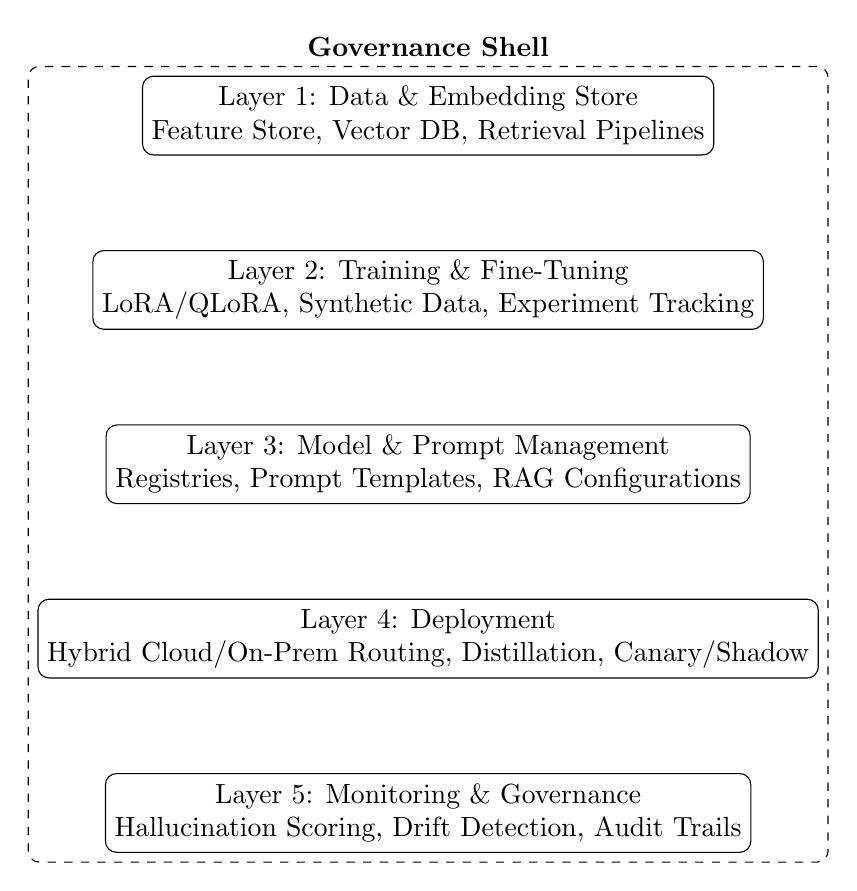
\begin{tikzpicture}[
    node distance=1.2cm,
    box/.style={rectangle, draw, rounded corners, minimum width=4cm, minimum height=1cm, align=center}
]

% Layers
\node[box] (data) {Layer 1: Data \& Embedding Store\\Feature Store, Vector DB, Retrieval Pipelines};
\node[box, below=of data] (train) {Layer 2: Training \& Fine-Tuning\\LoRA/QLoRA, Synthetic Data, Experiment Tracking};
\node[box, below=of train] (manage) {Layer 3: Model \& Prompt Management\\Registries, Prompt Templates, RAG Configurations};
\node[box, below=of manage] (deploy) {Layer 4: Deployment\\Hybrid Cloud/On-Prem Routing, Distillation, Canary/Shadow};
\node[box, below=of deploy] (monitor) {Layer 5: Monitoring \& Governance\\Hallucination Scoring, Drift Detection, Audit Trails};

% Governance shell
\node[draw, dashed, rounded corners, fit=(data)(train)(manage)(deploy)(monitor), label=above:{\textbf{Governance Shell}}] {};

\end{tikzpicture}
\caption{Unified MLOps + LLMOps Modernization Architecture}
\end{figure}


A governance shell surrounds the entire architecture, ensuring that every action—training, deployment, inference, and monitoring—is logged, auditable, and compliant with enterprise policy.

\section{Algorithms and Techniques for Enterprise LLMOps}

Operationalizing LLMs requires a blend of classical ML techniques and emerging generative AI methods. Key algorithms and techniques include:

\begin{itemize}[leftmargin=1.2cm]
    \item \textbf{Retrieval-Augmented Generation (RAG):} Grounding LLMs with enterprise knowledge sources.
    \item \textbf{Prompt Optimization and Caching:} Reducing inference cost by reusing optimized prompts.
    \item \textbf{Model Distillation and Quantization:} Creating lightweight variants for cost-sensitive workloads.
    \item \textbf{Embedding Drift Detection:} Monitoring semantic shifts in vector stores.
    \item \textbf{Hallucination Detection Models:} Scoring generative outputs for factual consistency.
    \item \textbf{Canary and Shadow Deployments:} Safely introducing new generative behaviors.
    \item \textbf{Reinforcement Learning for Automated Retraining:} Triggering fine-tuning based on drift signals.
\end{itemize}

These techniques form the operational backbone of enterprise-grade LLM systems.
\section{Implementation Considerations for Enterprise Deployment}

Enterprises rarely operate in greenfield environments. Most AI systems must coexist with legacy data warehouses, compliance frameworks, and infrastructure that predates modern ML tooling. For this reason, implementation strategy becomes as important as model architecture.

A practical deployment strategy begins with acknowledging organizational realities: fragmented data ownership, inconsistent DevOps maturity, and varying levels of GPU availability across business units. The modernization framework proposed here is intentionally adaptable. It does not assume a specific cloud provider or orchestration platform; instead, it outlines the principles required for a stable foundation.

\subsection{Infrastructure and Orchestration}

A robust orchestration layer is essential for managing both ML and LLM workloads. Kubernetes remains the de facto standard due to its portability and ecosystem maturity. On top of Kubernetes, enterprises typically adopt:

\begin{itemize}[leftmargin=1.2cm]
    \item \textbf{Kubeflow or MLflow} for pipeline orchestration and experiment tracking
    \item \textbf{Ray Serve} for distributed inference, especially for LLM workloads
    \item \textbf{Airflow} for scheduled data and feature engineering tasks
    \item \textbf{Vector databases} such as FAISS, Milvus, or Pinecone for retrieval pipelines
\end{itemize}

These components form a modular stack that can evolve as enterprise needs change.

\subsection{Security and Compliance}

LLMs introduce new security considerations. Unlike traditional ML models, which operate on structured datasets, LLMs may inadvertently expose sensitive information through prompts or generated outputs. Enterprises must enforce:

\begin{itemize}[leftmargin=1.2cm]
    \item Strict RBAC controls for model access
    \item Guardrail prompts to prevent leakage of confidential data
    \item Output filtering for compliance-sensitive domains
    \item Encryption of vector stores and embedding pipelines
\end{itemize}

Compliance is not a separate track—it is embedded throughout the lifecycle.

\subsection{Integration with Existing Systems}

Enterprises often underestimate the complexity of integrating LLMs into existing workflows. Successful integration requires:

\begin{itemize}[leftmargin=1.2cm]
    \item API gateways that unify ML and LLM inference endpoints
    \item Feature and embedding stores that share lineage metadata
    \item Monitoring dashboards that track both classical metrics and generative behaviors
    \item CI/CD pipelines that treat prompts, adapters, and RAG configurations as versioned artifacts
\end{itemize}

This integration ensures that LLMs do not become isolated prototypes but fully governed enterprise assets.

\section{Evaluation and Results}

Evaluating LLM systems requires a broader lens than traditional ML evaluation. Accuracy, precision, and recall remain relevant, but they are insufficient for generative systems. Enterprises must adopt a multi-dimensional evaluation strategy.

\subsection{Cost and Latency Benchmarks}

LLM inference cost is one of the most significant operational concerns. Extending the hybrid routing strategy from \textit{EfficientML-Cloud}, enterprises can achieve:

\begin{itemize}[leftmargin=1.2cm]
    \item 40--70\% reduction in inference cost through dynamic routing
    \item Predictable latency envelopes by shifting workloads between cloud and on-prem
    \item Improved GPU utilization through quantized and distilled model variants
\end{itemize}

These results demonstrate that cost-aware routing is as relevant for LLMs as it is for traditional ML models.

\subsection{Quality and Stability Metrics}

Generative quality must be measured using domain-specific criteria. Enterprises typically evaluate:

\begin{itemize}[leftmargin=1.2cm]
    \item Hallucination frequency and severity
    \item Semantic consistency with enterprise knowledge sources
    \item Toxicity and compliance adherence
    \item Retrieval accuracy for RAG pipelines
\end{itemize}

Embedding drift detection plays a critical role in maintaining long-term stability.

\subsection{Operational Reliability}

Operational reliability is measured by:

\begin{itemize}[leftmargin=1.2cm]
    \item Deployment cycle time (reduced from weeks to hours)
    \item Reproducibility of training and fine-tuning pipelines
    \item Frequency of drift-triggered retraining events
    \item Audit completeness for prompts, outputs, and model versions
\end{itemize}

These metrics reflect the maturity of the unified MLOps + LLMOps framework.

\section{Discussion}

Enterprises adopting LLMs face a unique set of trade-offs. High-capability models often come with high operational cost. On-prem deployments reduce latency but require significant infrastructure investment. Retrieval pipelines improve grounding but introduce new maintenance overhead.

The modernization framework presented here does not eliminate these trade-offs; instead, it provides a structured way to navigate them. By unifying MLOps and LLMOps, enterprises gain a consistent operational model that scales across use cases, departments, and regulatory environments.

A notable challenge is organizational readiness. Many enterprises underestimate the cultural shift required to operationalize LLMs. Prompt engineering, retrieval tuning, and generative evaluation require new skill sets that may not exist within traditional data science teams. Successful adoption requires cross-functional collaboration between engineering, compliance, security, and business stakeholders.

\section{Conclusion}

LLMs represent a transformative leap in enterprise AI capability, but they also introduce operational complexity that cannot be addressed with traditional MLOps alone. A unified MLOps + LLMOps modernization framework provides the structure needed to deploy, govern, and scale AI systems responsibly.

By extending principles from \textit{EfficientML-Cloud}—such as cost-aware routing, hybrid inference, and governance layers—enterprises can build AI systems that are not only powerful but predictable, auditable, and aligned with business constraints.

This paper outlines a practical, adaptable blueprint for organizations seeking to operationalize LLMs at scale. The path forward is not merely technical; it is organizational. Enterprises that embrace this unified framework will be positioned to lead in the next era of AI-driven innovation.






Hybrid inference reduces cost 
\cite{solan2026efficientmlcloud}
\cite{lewis2020rag}
\cite{chen2023llmops}
\cite{zhang2022governance}
\cite{openai2023bestpractices}
\cite{google2023embeddingdrift}
\bibliographystyle{apalike}
\bibliography{references}



\end{document}



